\documentclass[a4paper,11pt]{exam}
	\usepackage{graphicx}
	\usepackage[utf8]{inputenc}
	\usepackage[T1]{fontenc}
	\usepackage{listings}
	\usepackage{color}
	\usepackage{amsmath}
	\usepackage{enumerate}
	\usepackage{caption}
	\usepackage{verbatim}
	\usepackage{subcaption}
	\usepackage{tikz}
	\usepackage{graphics}
	\usepackage{txfonts}
	\usepackage{listings}
	\definecolor{dkgreen}{rgb}{0,0.5,0}
	\definecolor{gray}{rgb}{0.5,0.5,0.5}
	\definecolor{mauve}{rgb}{0.58,0,0.82}

	\lstset{frame=tb,
	  language=Python,
	  aboveskip=3mm,
	  belowskip=3mm,
	  showstringspaces=false,
	  columns=flexible,
	  basicstyle={\small\ttfamily},
	  numbers=none,
	  numberstyle=\tiny\color{gray},
	  keywordstyle=\color{blue},
	  commentstyle=\color{dkgreen},
	  stringstyle=\color{mauve},
	  breaklines=true,
	  breakatwhitespace=true
	  tabsize=3
	  }
\begin{document}
\begingroup 
	  \bf \Large Eletromagnetismo\\
	  \indent \normalsize André Del Bianco Giuffrida
	\endgroup
	\\ \quad
	\\
	\large{
	\emph{Lista 3 \\ Ex 4}
	\\
	\\
	\indent Uma carga pontual $q$ está localizada a uma distância $d$ com relação a um plano condutor infinito fixado a potencial zero. A referência de potencial está no infinito.
	\\
	\\
	\indent (a) Verifique que este problema real satisfaz as condições necessárias para obter o potencial $V(\vec{r})$ a partir da solução do problema imagem (com uma carga $-q$ a distância $2d$ da primeira): mesma $\rho$ e mesma condição de Dirichlet sobre o contorno S.
	\\
	\\
	\indent (b) Calcule a densidade de carga elétrica $\sigma$ sobre o plano condutor.
	\\
	\\
	\indent (c) É conveniente especificar condições de contorno de Neumann para este problema?
	\\
	\\
	\indent (d) Calcule a força que o plano exerce sobre a carga $q$.
	\\
	\\
	\indent (e) Calcule a energia eletrostática do sistema (carga e plano). 
	\\
	
	\normalsize
	\begin{center}
		\begin{tikzpicture}
			\node at (0,2.5) {Problema Real};
			
			\draw (0,-2) -- (0,2);
			\node at (-0.6,1) {$V=0$};
			
			\draw (0,-2) -- (0.2,-2);
			\draw (0.2,-2.2) -- (0.2,-1.8);
			\draw (0.3,-2.1) -- (0.3,-1.9);
			\draw (0.4,-2.05) -- (0.4,-1.95);
			
			\draw (2,0) -- (2,-0.9);
			\draw[arrows=<->] (0,-0.7) -- (2,-0.7);
			\node at (1,-1) {$d$};
			
			\draw[fill=black] (2,0) circle (0.1);
			\node at (2.4,0) {$q$};
			
			\draw[dashed] (5.5,-3.5) -- (5.5,3.5);
			
			\node at (10,2.5) {Problema Imagem	};
			\node at (7.6,0) {$-q$};
			\draw[fill=black] (8,0) circle (0.1);
			\node at (12.4,0) {$q$};
			\draw[fill=black] (12,0) circle (0.1);
			
			\draw (8,0) -- (8,-0.9);
			\draw[arrows=<->] (8,-0.7) -- (12,-0.7);
			\draw (12,0) -- (12,-0.9);
			\node at (10,-1) {$2d$};
			
		\end{tikzpicture}
	\end{center}
	
	(a)\\
	\indent No problema imagem podemos mostrar que $V(\vec{r})$ no plano a distância $d$ das duas cargas possui potencial $0$ devido a simetria do problema.
	\\
	\indent Resolvendo o problema real através do método das cargas imagens, podemos resolver para $q'$ e $d'$ a seguinte expressão:
	
	\[ V = 0 =\frac{1}{4 \pi \epsilon_0} \Bigg( \frac{q}{|\vec{r} - \vec{R}|} + \frac{q'}{|\vec{r} - \vec{R'}|} \Bigg)\]
	
	\indent Para a seguinte configuração:
	\begin{center}
		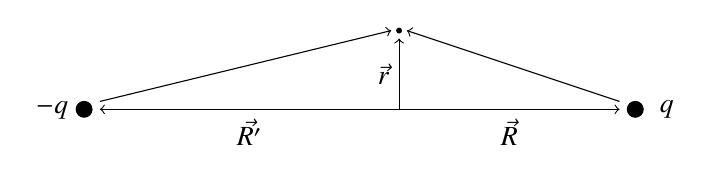
\begin{tikzpicture}
			\draw[fill=black] (0,1) circle (0.03);
			\draw[arrows=->] (0,0) -- (0,0.9) node[left,midway] {$\vec{r}$};
			\draw[arrows=->] (-3.8,0.1) -- (-0.1,1);
			\draw[arrows=->] (0,0) -- (2.8,0) node[below,midway] {$\vec{R}$};
			\draw[arrows=->] (2.8,0.1) -- (0.1,1);
			\draw[arrows=->] (0,0) -- (-3.8,0) node[below,midway] {$\vec{R'}$};
			\node at (-4.4,0) {$-q$};
			\draw[fill=black] (-4,0) circle (0.1);
			\node at (3.4,0) {$q$};
			\draw[fill=black] (3,0) circle (0.1);
		\end{tikzpicture}
	\end{center}
	\indent Pelo teorema da unicidade podemos ver que se, $q = -q'$ e $R = R'$ a expressão para o potencial é validada, e assim podemos obter o potencial do problema real através do potencial do problema imagem avaliado no semi-espaço do lado em que a carga real é situado, e o potencial do lado oposto é nulo, pois não exite caga e o potencial é contínuo, equalizando isso obtemos:
	
	\[V(\vec{r}) = 0 \quad \text{para} \quad x < 0 \]
	\[V(\vec{r}) = \frac{1}{4 \pi \epsilon_0} \Bigg( \frac{q}{|\,\vec{r}\, - d\,\hat{x}\,|} - \frac{q}{|\,\vec{r}\, + d\,\hat{x}\,|} \Bigg)\]
	
	\begin{figure}[h]
		\centering
		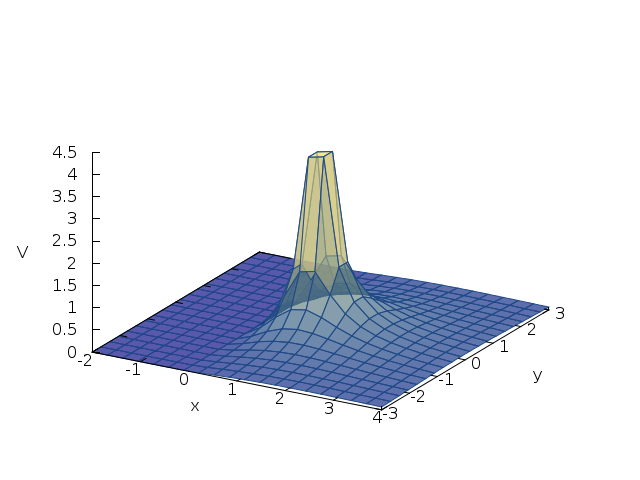
\includegraphics[scale=0.7]{V.png}
		\caption{ Potencial $V(\vec{r})$ no plano xy para a carga em (1,0,0) e o plano a potencial nulo em (0,y,z)}
	\end{figure}
	
	(b)
	\\
	\indent Para obter-mos $\sigma$ podemos partir do potencial já encontrado e calcular o campo elétrico $\vec{E}$.
	\[\vec{E} = - \nabla V(\vec{r}) \quad \text{e pelas condições de contorno} \quad \big( \vec{E_1} - \vec{E_2} \Big)\cdot\hat{n} = \frac{\sigma}{\epsilon_0} \]

	\[ 4 \pi \epsilon_0 \, \vec{E_1} = -\frac{\partial }{\partial x} \Bigg( \frac{q}{|\,\vec{r}\, - d\,\hat{x}\,|} - \frac{q}{|\,\vec{r}\, + d\,\hat{x}\,|} \Bigg) - \frac{\partial }{\partial y} \Bigg( \frac{q}{|\,\vec{r}\, - d\,\hat{x}\,|} - \frac{q}{|\,\vec{r}\, + d\,\hat{x}\,|} \Bigg) - \frac{\partial }{\partial z} \Bigg( \frac{q}{|\,\vec{r}\, - d\,\hat{x}\,|} - \frac{q}{|\,\vec{r}\, + d\,\hat{x}\,|} \Bigg) = \]
	
        \[\vec{E_1} = \frac{-1}{4 \pi \epsilon_0} \Bigg( \frac{ q (x+d) \, \hat{x} + y \, \hat{y} + z \, \hat{z}}{\Big((x+d)^2 + y^2 + z^2 \Big)^{3/2}} \Bigg)\]
	
	\[\vec{E_2} = 0 \quad \text{pois o potencial é constante e nulo em } \, x<0\]
	
	\[\vec{E} \cdot \hat{x}  = \frac{-1}{4 \pi \epsilon_0} \Bigg( \frac{q(x+d)}{\Big((x+d)^2 + y^2 + z^2 \Big)^{3/2}} \Bigg) \Bigg|_{x=0}\]
	
	Assim obtemos $\sigma$ no plano $x=0$:
	
	\[\ \sigma = -\frac{1}{4 \pi} \Bigg( \frac{q\,d}{\Big(d + y^2 + z^2 \Big)^{3/2}} \Bigg)\] 
	
	\begin{figure}[h]
		\centering
		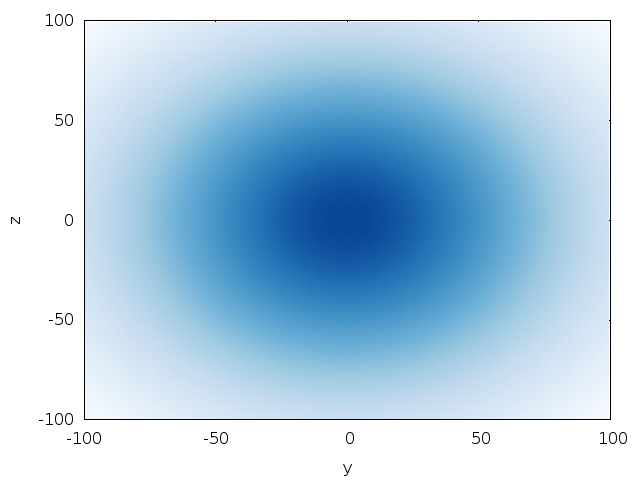
\includegraphics[scale=0.7]{Sigma.png}
		\caption{ Densidade superficial de carga $\sigma$ no plano $x=0$ em frente a carga}
	\end{figure}
	(c)
	\\
	As Condições de Contorno de Neumann, implicam em fornecer a variação na direção normal do potencial na superfície ao invés de fornecer $V(r)$ no contorno explicitamente, como fizemos no início (Condição de Contorno de Dirichlet).
	\[\frac{\partial V(\vec{r})}{\partial n} \Bigg|_s \to \text{é dado!}\quad \to \quad \text{Condição de Contorno de Neumann} \]
	\[V(\vec{r}) \Bigg|_s \to \text{é dado!}\quad \to \quad \text{Condição de Contorno de Dirichlet} \]
	
	(Pensar melhor sobre isso!)
	
	(d)
	A força que o plano exerce sobre a carga, pode ser feita integrando a densidade de carga, porém podemos calcular através do problema imagem, pois a força que o plano exerce sobre a carga é a força que atua na carga, e é a mesma para o problema imagem , como no esquema:
	
	\begin{center}
		\begin{tikzpicture}
			\node at (0,2.5) {Problema Real};
			
			\draw (0,-2) -- (0,2);
			\node at (-0.6,1) {$V=0$};
			
			\draw (0,-2) -- (0.2,-2);
			\draw (0.2,-2.2) -- (0.2,-1.8);
			\draw (0.3,-2.1) -- (0.3,-1.9);
			\draw (0.4,-2.05) -- (0.4,-1.95);
			
			\draw (2,0) -- (2,-0.9);
			\draw[arrows=<->] (0,-0.7) -- (2,-0.7);
			\node at (1,-1) {$d$};
			
			\draw[fill=black] (2,0) circle (0.1);
			\node at (2.4,0) {$q$};
			
			\draw[arrows=->] (0,0) -- (0.5,0) node[above,midway] {$\vec{F}$};
			\draw[arrows=->] (2,0) -- (1.5,0) node[above,midway] {$-\vec{F}$};
			
			\draw[dashed] (5.5,-3.5) -- (5.5,3.5);
			
			\node at (10,2.5) {Problema Imagem	};
			\node at (7.6,0) {$-q$};
			\draw[fill=black] (8,0) circle (0.1);
			\node at (12.4,0) {$q$};
			\draw[fill=black] (12,0) circle (0.1);
			
			\draw[arrows=->] (8,0) -- (8.5,0) node[above,midway] {$\vec{F}$};
			\draw[arrows=->] (12,0) -- (11.5,0) node[above,midway] {$-\vec{F}$};
			
			\draw (8,0) -- (8,-0.9);
			\draw[arrows=<->] (8,-0.7) -- (12,-0.7);
			\draw (12,0) -- (12,-0.9);
			\node at (10,-1) {$2d$};
			
		\end{tikzpicture}
	\end{center}
	
	\indent É necessário que as forças sejam as mesmas, os dois problemas são identicos para $x>0$, ou seja, a força que atua na carga $q$ é a mesma que atua na carga $q'$ no problema imagem e é a mesma no problema real que atua sobre o plano.\\
	\indent A força de Coulomb para as duas cargas é $\vec{F}$ e é a mesma força para a carga em frente ao plano.
	\[\vec{F} = -\frac{q^2}{16 \pi \epsilon_0 d^2} \hat{x}\]
	\\
	(e)
	\\
	Para calcular a energia eletrostática armazenada no sistema podemos partir da definição de trabalho $W$ e assim podemos encontrar a variação da energia potencial elétrica calculando o trabalho para trazer a carga $q$ do infinito até a distância $d$ do plano.
	\[ W_{ab} = \int_a^b \vec{F} \cdot \, d\vec{l} = \Delta U_{ab}  \]
	
	No problema real a densidade de carga no plano vai variar com a distância da carga ao plano, porém é muito mais fácil olhar-mos como varia a força no problema imagem, assim podemos concluir que é necessário trazer a carga imagem ao mesmo tempo que a carga real para que a condição de contorno seja satisfeita ($V=0$ em $x=0$), assim podemos calcular a força na carga $q$ a distância $2x$ da carga $-q$.
	\[ \vec{F} = \frac{-q^2}{4\pi\epsilon_0 (2x)^2} \]
	\begin{center}
		\begin{tikzpicture}
			\draw[dashed] (0,-0.3) -- (0,0.5) node[above] {$V=0$};
			\draw[dashed] (0,-1.1) -- (0,-1.5) node[below] {$\sigma(x)$};
			\draw (3,0) -- (3,-0.9);
			\draw (-3,0) -- (-3,-0.9);
			\draw[arrows=<->] (-3,-0.5) -- (3,-0.5) node[below,midway] {$2x$};
			\draw[fill=black] (3,0) circle (0.1) node[right] {$q$};
			\draw[fill=black] (-3,0) circle (0.1) node[left] {$-q$};
		\end{tikzpicture}
	\end{center}
	Fazendo a integral temos:
	\[W = \int_{\infty}^d \frac{-q^2}{16 \pi\epsilon_0 x^2} dx = \frac{q^2}{16 \pi\epsilon_0}\int_d^{\infty} \frac{1}{x^2} dx\]
	\[W =  \frac{-q^2}{16 \pi\epsilon_0 d} \]
\end{document}
